\section{Linear sufficiency and reliability}
\label{sec:sufficiency}

Write $K=(A,B)=S+N$ for a latent signal $S$ and independent measurement noise $N$, with covariances $\Sigma_S$ and $\Sigma_N$.
Let $\Sigma_K=\Sigma_S+\Sigma_N$.
An outcome margin $M=b^\top S+\varepsilon$ yields the binary label $Y=\ind\{M>0\}$, with coefficient $b=(b_A,-b_B)$ and independent noise $\varepsilon$.
Write $c=(1,-1)$, so $D=c^\top K$.
Let $\beta=\Sigma_K^{-1}\Sigma_S b$ be the best linear predictor of $M$ from $K$, and write $R^2_{\mathrm{full}}$ and $R^2_D$ for the population coefficients of determination of $(A,B)$ and of $D$.

\begin{theorem}[Alignment]
\label{thm:alignment}
\[
  \frac{R^2_D}{R^2_{\mathrm{full}}}
  = \cos^2\theta_K,
  \qquad
  \cos\theta_K
  = \frac{c^\top\Sigma_K\beta}{\sqrt{c^\top\Sigma_K c}\,\sqrt{\beta^\top\Sigma_K\beta}}.
\]
Equality holds if and only if $\beta\propto c$.
\end{theorem}

\begin{proof}
The linear predictor of $M$ from $D$ is the projection of $\beta$ onto $\operatorname{span}\{c\}$ in the $\Sigma_K$ inner product.
Its squared length is $(c^\top\Sigma_K\beta)^2/(c^\top\Sigma_K c)$, while $\|\beta\|_{\Sigma_K}^2=\beta^\top\Sigma_K\beta$.
Cauchy--Schwarz therefore gives the displayed cosine, with equality precisely when $\beta\propto c$.
The identity $c^\top\Sigma_K\beta=c^\top\Sigma_S b$ follows from $\beta=\Sigma_K^{-1}\Sigma_S b$.
\end{proof}

Thus $D$ is a \emph{linearly} sufficient feature precisely when the population coefficient aligns with $(1,-1)$.
The condition $b_A=b_B$ is neither necessary nor sufficient for that alignment once $\Sigma_S$ or $\Sigma_N$ is asymmetric.
\Cref{fig:alignment} plots the alignment ratio against the angle between $\beta$ and $c$ in the $\Sigma_K$ inner product.

\begin{figure}[t]
  \centering
  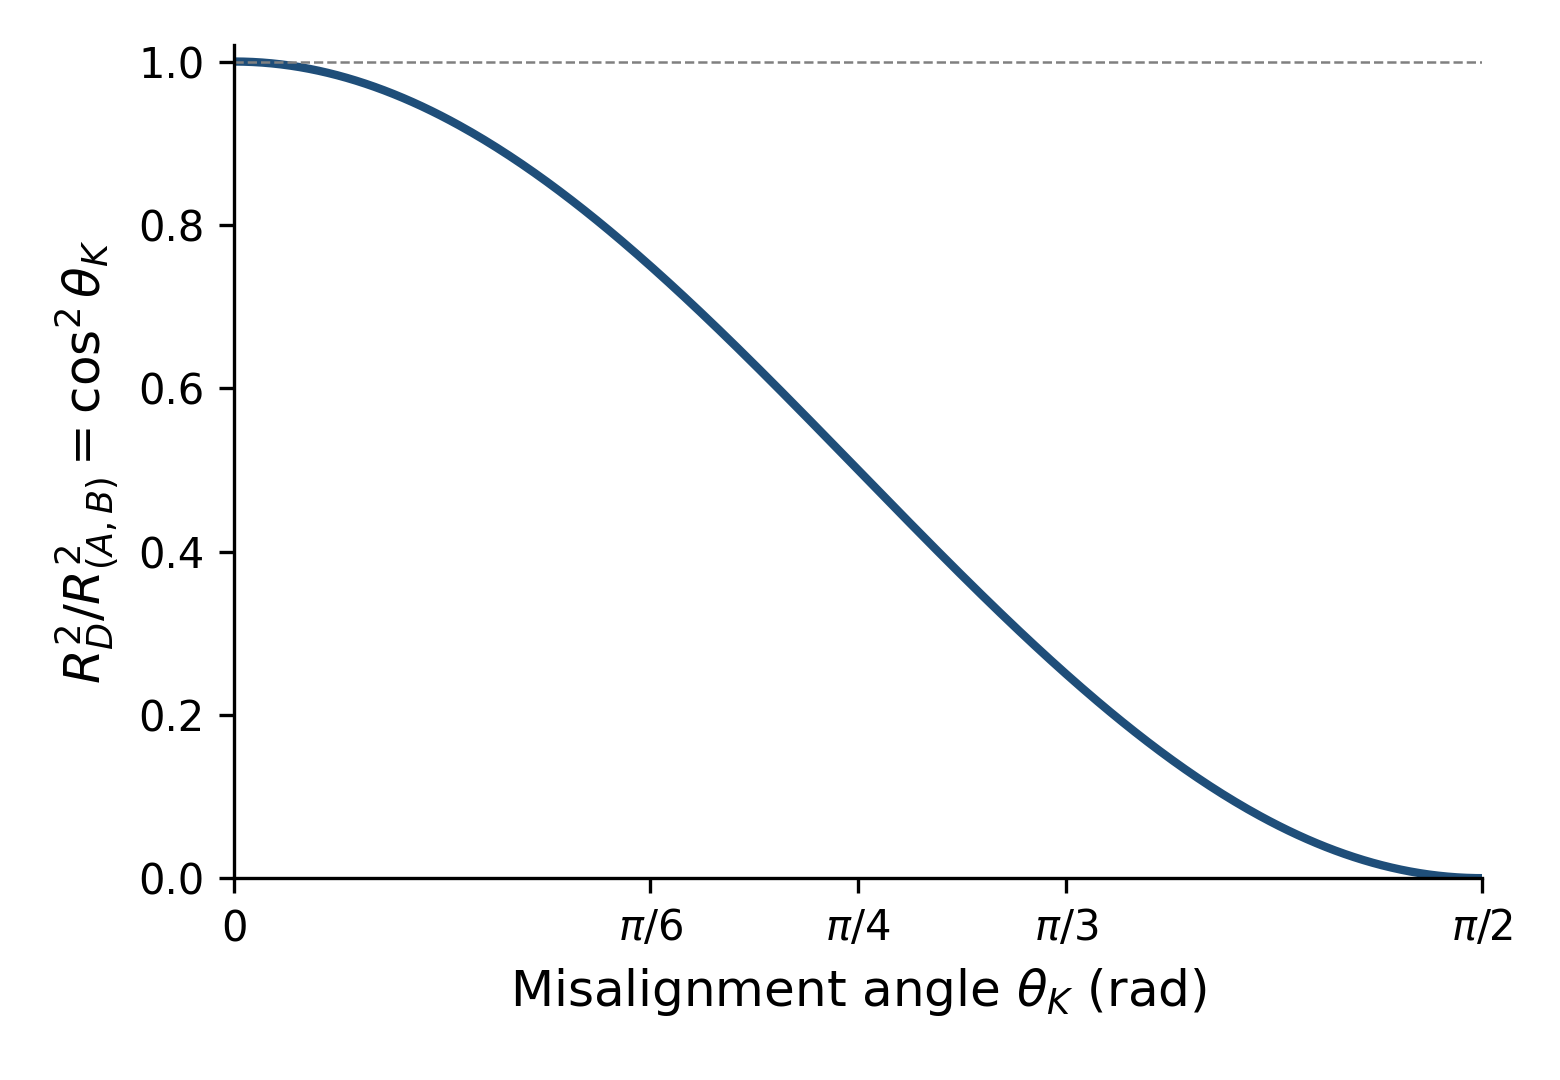
\includegraphics[width=0.72\linewidth]{figures/Figure_1_alignment_ratio.png}
  \caption{Alignment ratio $R^2_D/R^2_{(A,B)}=\cos^2\theta_K$ as a function of the misalignment angle between $\beta$ and $c=(1,-1)$.
           The identity is algebraic; the curve is not a simulation.}
  \label{fig:alignment}
\end{figure}

\begin{lemma}[Probit and logistic coefficients]
\label{lem:bridge}
Under joint normality of $(K,M)$,
\[
  P(Y=1\mid K)
  = \Phi\!\left(\frac{\mathbb{E}[M\mid K]}{\sqrt{\Var(M\mid K)}}\right),
\]
and $\mathbb{E}[M\mid K]$ is linear in $K$ with coefficient $\beta$.
Probit coefficients on $(A,B)$ are therefore proportional to $\beta$.
Logistic coefficients are approximately so when the probit and logit links are close on the fitted scale.
\end{lemma}

Under joint normality, Bayes log-loss, Brier score, AUC and mutual information for any linear index depend on the pair $(z,r^2)$ alone, where $z=\mathbb{E}[M]/\sqrt{\Var(M)}$ and $r^2$ is the relevant coefficient of determination~\parencite{falconer1965,lee2012}.
Comparing feature sets then reduces to comparing $R^2$, and linear sufficiency becomes full sufficiency for $Y$.
Outside the Gaussian case, \cref{thm:alignment} remains a statement about $R^2$ only.

The ratio of $R^2_D$ to the single-entity coefficient $R^2_A$ is, in general,
\begin{equation}
  \frac{R^2_D}{R^2_A}
  = \frac{(c^\top\Sigma_S b)^2}{(e_A^\top\Sigma_S b)^2}
    \cdot
    \frac{(\Sigma_K)_{AA}}{c^\top\Sigma_K c},
  \label{eq:r2_ratio_general}
\end{equation}
where $e_A=(1,0)^\top$.
When $\kappa_S=\kappa_N=b_{\mathrm{ratio}}=1$, with $b_{\mathrm{ratio}}=b_B/b_A$, this reduces to
\begin{equation}
  \frac{R^2_D}{R^2_A}
  = 2\eta,
  \label{eq:r2_ratio_exchangeable}
\end{equation}
and $\eta$ is computed from the total feature correlation.
Outside that exchangeable case the factor $2\eta$ does not hold.

A single value of $\eta$ does not fix $R^2_D$.
\Cref{tab:eta2} stores three designs with total $\eta=2$ and $R^2_D$ equal to $0.80$, $0.33$ and $0$.
The zero case has $c^\top\Sigma_S b=0$ while $\Sigma_K=\Sigma_S+\Sigma_N$ still yields $\eta=2$.

\begin{table}[t]
  \centering
  \caption{Three designs with $\eta=2$ and distinct $R^2_D$.
           Entries are the exact population parameters from the stored counterexample.}
  \label{tab:eta2}
  \begin{tabular}{@{}lcccc@{}}
    \toprule
    Case & $\Sigma_S$ & $\Sigma_N$ & $b$ & $R^2_D$ \\
    \midrule
    High &
      $\begin{pmatrix}1&0.2\\0.2&1\end{pmatrix}$ &
      $\begin{pmatrix}1&0.8\\0.8&1\end{pmatrix}$ &
      $(1,-1)$ & $0.80$ \\
    Mid &
      $\begin{pmatrix}1&0.67\\0.67&1\end{pmatrix}$ &
      $\begin{pmatrix}1&0.33\\0.33&1\end{pmatrix}$ &
      $(1,-1)$ & $0.33$ \\
    Zero &
      $\begin{pmatrix}0.5&0.5\\0.5&0.5\end{pmatrix}$ &
      $\begin{pmatrix}1&0.25\\0.25&1\end{pmatrix}$ &
      $(1,0)$ & $0$ \\
    \bottomrule
  \end{tabular}
\end{table}

Reliability of $D$ is decided by the split of pairing efficiency between signal and noise, not by total $\eta$.
Write $S_D=S_A-S_B$, $N_D=N_A-N_B$, $\nu=\operatorname{tr}\Sigma_N/\operatorname{tr}\Sigma_S$, and let $\eta_S$ and $\eta_N$ be the Paired Efficiency Factors of the signal and noise components.

\begin{theorem}[Reliability]
\label{thm:reliability}
\[
  \Rel(D)
  = \frac{\Var(S_D)}{\Var(D)}
  = \frac{1}{1+\nu\,\eta_S/\eta_N}.
\]
\end{theorem}

\begin{proof}
With $S\perp N$, one has $\Var(D)=\Var(S_D)+\Var(N_D)$.
For any $2\times 2$ covariance $\Sigma$, $\Var(c^\top X)=\operatorname{tr}\Sigma/\eta(\Sigma)$, so $\Var(S_D)=\operatorname{tr}\Sigma_S/\eta_S$ and $\Var(N_D)=\operatorname{tr}\Sigma_N/\eta_N$.
Substituting $\nu=\operatorname{tr}\Sigma_N/\operatorname{tr}\Sigma_S$ gives the displayed ratio.
\end{proof}

The identity uses second moments only.
When $b=c$, one has $R^2_D=\Rel(D)\cdot q$ with outcome determinism $q=\Var(S_D)/\Var(M)$, the classical attenuation identity~\parencite{fuller1987}.
Relativisation therefore multiplies the pair-level noise-to-signal ratio by $\eta_S/\eta_N$.
It does not, by itself, decide alignment.
